\subsection{Design one}
This design revolves around the user being able to customize almost everything. The design therefore aims to be very flexible, and to accommodate almost every situation.

\subsubsection*{Description}
The user in this design will be given 3 or more stickers of different colours. See figure \ref{fig:wheel}. In this example, a red, green and a blue sticker are used, but since the design is so customizable, the user should be given the ability to choose colours him/herself. The user can also make the stickers themselves, in which case the design is completely free for the user.


\begin{figure}[h]
\centering
\subfigure[example sticker configuration.]{\label{fig:design11}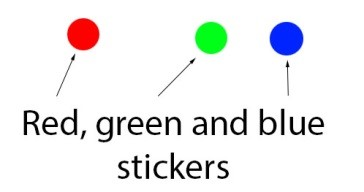
\includegraphics[scale=1]{Design11}}
\subfigure[Object for steering with stickers on.]{\label{fig:design12}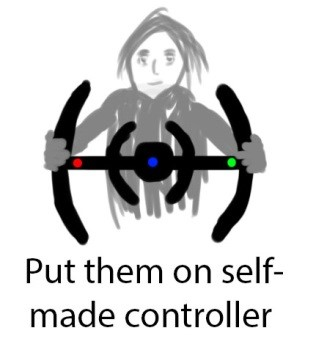
\includegraphics[scale=1]{Design12}}
\caption{Sticker configuration.}\label{fig:wheel}
\end{figure}

The user then places these stickers on some object he/she would like to use as a mean of controlling a vehicle inside a game. In this example, the stickers are placed on a steering wheel, which could be cut out from cardboard.

\begin{figure}[h]
\centering
\subfigure[example of what the menu for steering could look like.]{\label{fig:design14}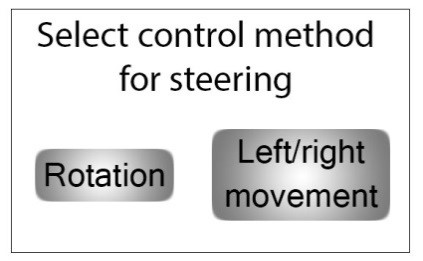
\includegraphics[scale=1]{Design14}}
\subfigure[example of what the menu for acceleration could look like.]{\label{fig:design13}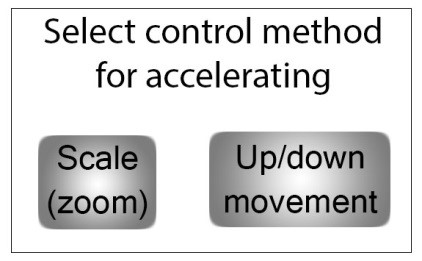
\includegraphics[scale=1]{Design13}}
\caption{Menu examples.}\label{fig:select}
\end{figure}

The user then picks how he/she would like to use the object for steering. Only two options are listed in this example, but more could be added, including ways of customizing the control method e.g. for example, choosing how much you should be able to rotate the controller before reaching the maximum turning speed. See figure \ref{fig:select}.

\bigskip

Customization is also allowed for acceleration in which case the user can choose between moving the controller closer or further away from the camera, moving the controller up and down, or moving one hand up or down separately from the steering wheel. 
The acceleration itself would simply change between max acceleration and no acceleration at all, or acceleration, no acceleration, and breaking, for simplicity. A separate sticker placed inside one’s hand can be used for braking, if it is needed to brake and use the speeder at the same time.

\bigskip

Gear shifting can be set up by being the “opposite” of controlling the speed. So if the user chooses to use up/down movement of the controller for speed, the user can use his/her free hand to separately control the gear shift. If the user holds their hand, with stickers attached, high, it would change the gear up, if the user holds it low, change the gear down, and if it’s in the center area, do not change gear. See figure \ref{fig:design15} for example of rotation and gear shift.

\begin{figure}[h]
\centering
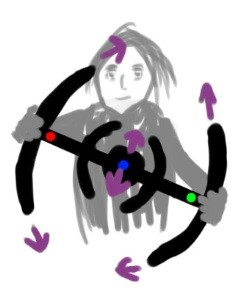
\includegraphics[scale=1]{Design15}
\caption{Controller in use.}
\label{fig:design15}
\end{figure}

To implement an extra action such as using power-ups or something similar, the opposite of the steering control method could be used. If the user is using rotation for steering, left/right movement could be used for extra action functionalities, and vice versa if the user chose left/right movement for steering.
After everything is set up, the user now has his/her own custom-made controller, unlike any other. He/she can use it to control vehicles inside game, only needing a webcam to pick up the colours, and a computer. In this example, the control method for steering is rotation, so the user would use the object as a form of steering wheel. The method for acceleration is scale/zoom, so the user will have to move towards/away from the camera in order to accelerate and brake.
\bigskip

This design will output the users commands as simulated presses to the keyboard. 
Because the keyboard mappings differ from game to game, the individual keys that should be simulated by the software will be provided to the software by a profile.
The profile will contain a mapping of the command types to the keys that should be simulated. 
The software should have no interaction with the game other than the simulated keyboard presses.

\subsubsection*{Compared to the FPS and List of Requirements}
The FPS is focused on creating a cheap alternative to already existing vehicle controllers. This design not only creates a solution that needs nothing else than a standard laptop, it also lets the user specify and control almost every aspect of controlling, and lets them create their own controller. It is not even necessary to make a controller; the user can paint their hands and use them instead if they want.

Compared to the list of requirements, this design fulfills everything but the ability to brake while accelerating, nor gear shifting. In the example explained, it also does not fulfil the ability for extra action buttons. However the design can be made more complete to allow such control methods, without the need of additional purchases, such as buttons, by adding customization options to the user.


\pagebreak[2]
\subsubsection*{Pros and Cons}
Pros:
\begin{itemize}
\item It is free of cost, provided the user has a computer and webcam.
\item Potentially adds an infinite number of customization options.
\item It is not limited to a single game.
\end{itemize}
Cons:
\begin{itemize}
\item The amount of setting-combinations could potentially be complicated for the user.
\item It could, be potentially, hard to make.
\end{itemize}

\subsubsection*{Image processing usage}
In the example mentioned earlier, colour tracking is used to track the rotation. This would probably be the simplest and easiest way to make the design, however not everyone will be able to use the design if colour tracking is used, since it limits what colours are allowed to be worn by the user, and what colours are in the background.

Potentially, pattern recognition or template matching could be used instead. In that case, the user should be able to wear whatever colours they want, and the background can include any colour as well. Another customization option could also be added with this, so the user could choose whether to use colour tracking or pattern recognition.

A simple version of this could easily be created, simply by removing most of the customization options.
